\subsection{Bayesian Inference}
The Bayesian inversion approach samples a posterior distribution of depth profiles. For comparison to the other inversion methods, we consider only the depth at each grid point which corresponds to the maximum of the posterior probability distribution at that point. This is achieved by taking the maximum of the kernel density of the estimated depth distribution at each point along the 1D profile. 

This method is first applied using synthetic $k$ input and the resulting depth estimate is shown in Figure~\ref{mcmc-synthetic}. As for other methods, the synthetic result accurately represents the sandbar located at $x~\sim~950~m$ along the profile, which is an important feature to recreate. However, at offshore locations ($x~<~600~m$), the estimation appears to break down. As in other methods, this is expected because of the lower sensitivity of $k$ on $h$ at these depths, a relationship on which our inverse methods rely.


\begin{figure}[H]
\center
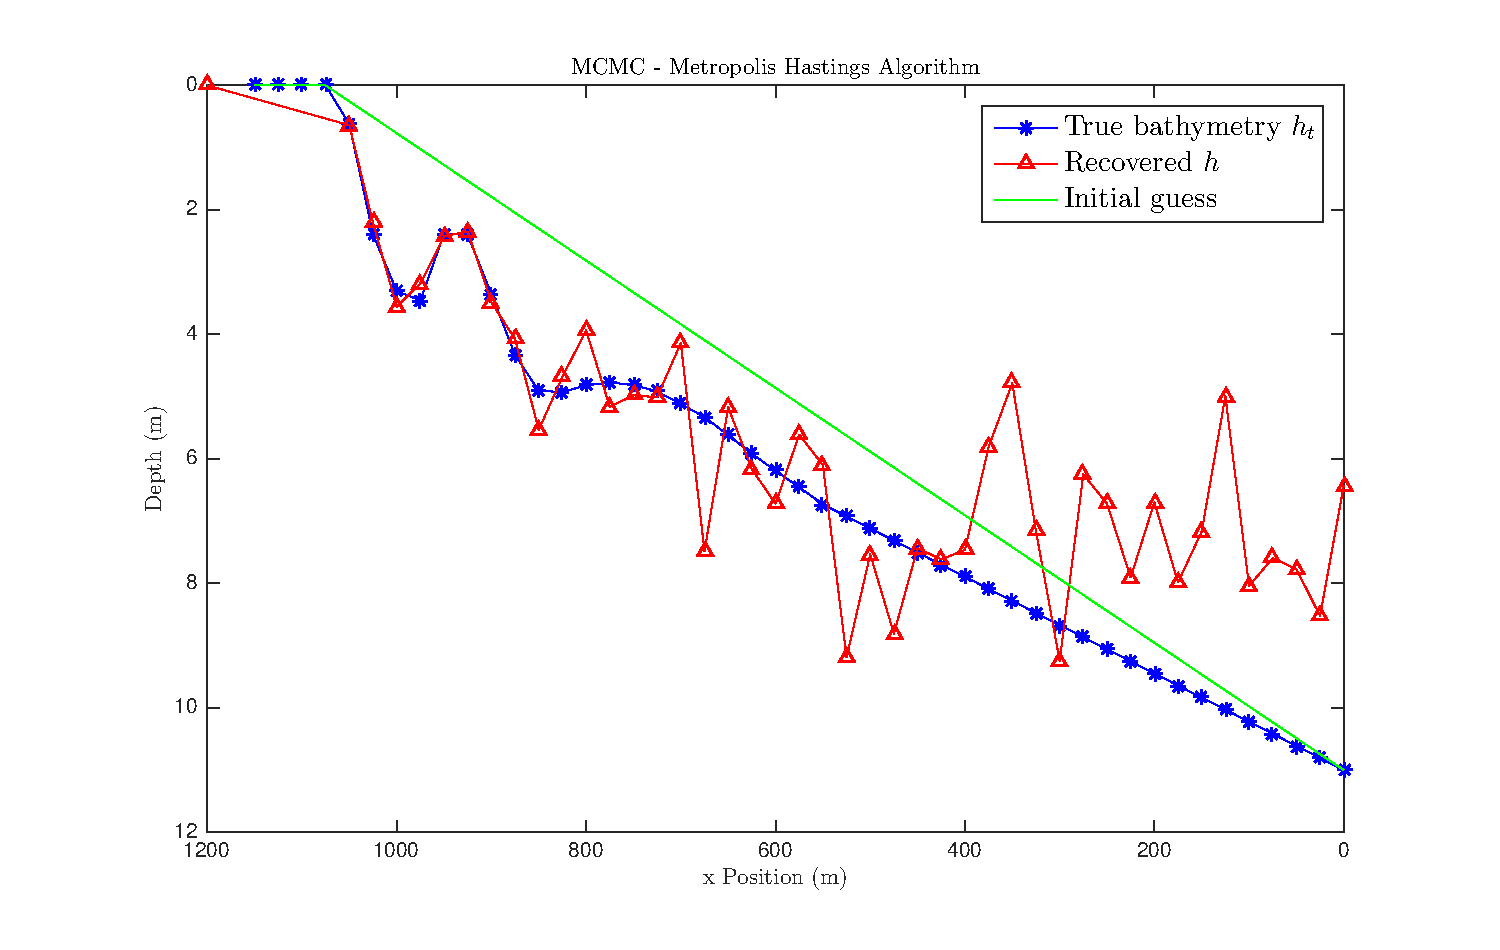
\includegraphics[scale=0.46]{img/MCMC-manufactured.eps} %plot20 
\caption{Bathymetry estimate from the Bayesian Markov Chain Monte Carlo approach. The initial $h$ guess is shown in green, the true $h$ is shown in blue, and the derived estimate of $h$ is shown in red.}
\label{mcmc-synthetic}
\end{figure}

Real $k$ data is then used to estimate the same bathymetry profile (Figure~\ref{mcmc-real}). We find...


Unlike the other methods, the Bayesian approach results in a distribution of depth profiles which optimize $h$ given uncertain $k$. Measurements of wave number, $k$, are not perfect and our resulting distribution of depth profiles translates that uncertainty binto an ensemble of depth estimates which are consistent with the $k$ data to within uncertainty. Figures~\ref{mcmc-posterior-h-synthetic} and \ref{mcmc-posterior-h-real} show the resulting posterior depth distributions. Note that...



